%dus was ik aan het nadenken over de stand van zaken na dynbenchmark ─ oké, ik heb zin om een dynbenchmark2 te doen moet, alles meer en beter
%maar hoe hebben we een impact gehad? als je kijkt naar course material over trajectory inference zou ik zeggen, veel ─ we zijn een gemakkelijke bron van guidelines
%maar als ik kijk naar de manuscripten van nieuwe TI methoden zou ik zeggen dat we nog niet zijn waar we wouden geraken

\section{Self-assessment in trajectory inference}
Many trajectory inference (TI) tools lack quantitative assessment of the accuracy of the method. Instead, they rely on anecdotal evidence to demonstrate their added value. A brief review of 76 TI articles reveals that only about 35\% contain a self-assessment (Figure \ref{fig:benchmarks_over_time}). Peer-reviewed TI articles fared even worse, self-assessing in only 32\% of cases (n=52), whereas articles first published as a pre-print self-assess in 42\% of cases (n=40). Only four TI articles feature a decently-sized comparison of at least 5 methods using 5 datasets or more.
% Note: i did not count how many metrics each of these manuscripts used.

Self-assessments are universally biased in favour of the authors, intentionally or otherwise, but this does not mean they should be skipped out on. Norel et al. provide a valuable discussion on overcoming overly optimistic self-assessments \cite{norel_selfassessmenttrapcan_2011}.
% TODO: improve working "this does not mean they should be skipped out on"

In this perspective, we hypothesise that low self-assessment rates are primarily caused by a lack of a standardised problem definition, benchmarking datasets, and metrics. 
We elaborate on these reasons and viable solutions to easy benchmarking trajectory inference.

%in deze commentary geven we nog een kort overzicht van:
%* standaard definitie van een trajectory inference probleem
%* waar kan je datasets vinden (dynbenchmark zenodo, de verschillende simulatoren, of download ze zelf van GEO)
%* hoe kan je methoden vergelijken (i.e. gebruik dynmethods)
%* wat zijn bestaande metrieken (toon overzicht van metrieken uit verschillende benchmarks en ook die van dyneval)

\begin{figure}[htb!]
	\centering
	\includegraphics[width=.75\linewidth]{fig/self_assessment.pdf} 
	\caption{\textbf{The number of manuscripts featuring trajectory inference tools over time.} Areas coloured in darker shades of blue represent manuscripts containing self-assessment of the tool, highlighting \textbf{A}: the number of datasets used and \textbf{B}: the number of methods used (including the method of the authors).}
	\label{fig:benchmarks_over_time}
\end{figure}

\subsection{Problem definition}
One main reason why benchmarking TI methods is difficult is due to there being slight variations 
of the problem a method is attempting to solve (Figure \ref{fig:method_types}A). For example, a method might infer linear or cyclic trajectories, or predict the probability of a cell ending up in one of several end states.

\begin{figure}[htb!]
	\centering
	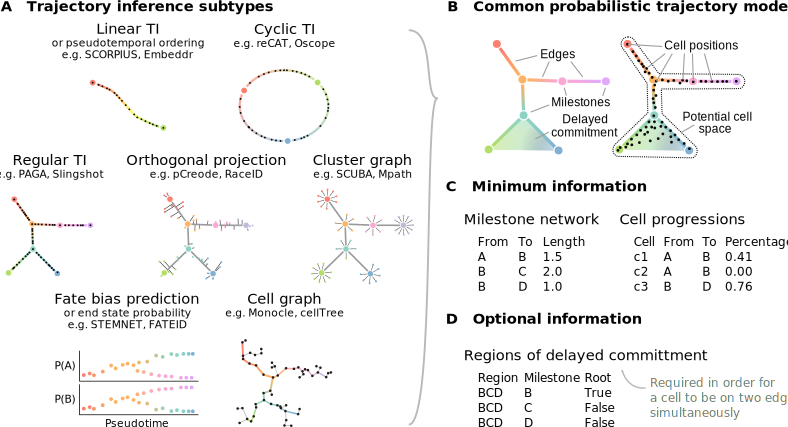
\includegraphics[width=.8\linewidth]{fig/method_types.pdf} 
	\caption{\textbf{Different forms of trajectory inference cause }.}
	\label{fig:method_types}
\end{figure}

As a result, it becomes harder to discover similar methods to compare against, as certain articles might only show up with search terms such as "pseudotemporal ordering", "lineage trees" or "fate bias". For the discoverability of a new TI method, it is therefore essential to use the term "trajectory inference", or at least list it as one of the keywords. 

A more significant and harder to solve problem is that the data formats produced by different methods varies greatly. This makes visualising and comparing multiple trajectories difficult, as different output types cannot be compared directly. The most commonly used and general is one where cells are positioned along a set of edges connecting milestones (Figure~\ref{fig:method_types}B). In practice, this format consists of two data structures: the milestone network specify transition between cell states, and the cell progressions specify how far along each cell has progressed along a transition (Figure~\ref{fig:method_types}C). Optionally, a cell can be in a region of "delayed commitment", that is, it is not known which state will end up in but a probability for ending up in either state can be assigned (Figure~\ref{fig:method_types}D). 

Saelens et al. \cite{saelens_comparisonsinglecelltrajectory_2019} developed an R package, \texttt{dynwrap}, for converting many of the variations of trajectory inference to the common format. Using this standardised format allows developing reusable software for interpreting, comparing, and visualising trajectories from any TI method.

\subsection{Benchmarking datasets}

\subsection{Multiple metrics}

%waarom benchmarks maar een laag aantal datasets hebben: 
%* echte datasets zijn duur om te genereren
%* het is niet evident om ze te verzamelen
%* otoh, we zouden naar de meta-informatie van de dynbenchmark/real datasets kunnen kijken en een cumulatieve plot genereren van hoeveel datasets er beschikbaar zijn over tijd, om aan te tonen dat sinds 2016-2017 er feitelijk wel al genoeg datasets zijn om aan self-benchmarking te doen

%waarom benchmarks een laag aantal methoden hebben:
%* iedere methode heeft zijn eigen set van functies
%* methodes hebben vaak andere prior inputs (starting cell, time series, etc)
%* methodes zijn vaak in verschillende talen geschreven (R, python, matlab)
%* de output van methodes zijn vaak niet rechtstreeks vergelijkbaar, omdat er geen standaard definitie van wat trajectory inference is (zoals bv. wel het geval is bij clustering of differential expression)
%
%bovendien is trajectory inference een probleem met complexe output, waardoor geen kant-en-klare metrieken bestonden om de predicties mee te evalueren. ik zou nog eens door alle manuscripten die een evaluatie hebben gedaan, moeten gaan, maar ik denk dat alle of toch de meeste evaluaties tussen 2016 en 2018 enkel op basis van pseudotime zijn ─ ook voor bv. dpt, en dat er maar zelden evaluaties zijn die echt gaan kijken naar de branching
%
%
%kaart aan dat we in 2018 een benchmark preprint hebben gepost van W methoden op X datasets, en in 2019 een artikel hebben gepubliceerd van Y methoden op Z datasets. Ondanks dat we in deze manuscripten de grootste problemen (# datasets, # methodes, # metrieken, leg iets beter uit) aanpakken, zien we geen vermindering in het aantal nieuwe publicaties die geen self-benchmark bevatten.
%in deze commentary geven we nog een kort overzicht van:
%* standaard definitie van een trajectory inference probleem
%* waar kan je datasets vinden (dynbenchmark zenodo, de verschillende simulatoren, of download ze zelf van GEO)
%* hoe kan je methoden vergelijken (i.e. gebruik dynmethods)
%* wat zijn bestaande metrieken (toon overzicht van metrieken uit verschillende benchmarks en ook die van dyneval)
%in conclusie, met al deze informatie melden we dat in 2019 er dus geen enkele reden is om ons te gedragen als gelijk welk ander computationeel / data mining / machine learning veld waarbij er voor quantitatief bewijs wordt gevraagd dat je methode goed werkt als je een nieuwe methode wilt publiceren. we vragen vriendelijk aan peer-reviewers om kritisch te zijn over deze kwestie.

%in deze commentary geven we nog een kort overzicht van:
%* standaard definitie van een trajectory inference probleem
%* waar kan je datasets vinden (dynbenchmark zenodo, de verschillende simulatoren, of download ze zelf van GEO)
%* hoe kan je methoden vergelijken (i.e. gebruik dynmethods)
%* wat zijn bestaande metrieken (toon overzicht van metrieken uit verschillende benchmarks en ook die van dyneval)

%in conclusie, met al deze informatie melden we dat in 2019 er dus geen enkele reden is om ons te gedragen als gelijk welk ander computationeel / data mining / machine learning veld waarbij er voor quantitatief bewijs wordt gevraagd dat je methode goed werkt als je een nieuwe methode wilt publiceren. we vragen vriendelijk aan peer-reviewers om kritisch te zijn over deze kwestie.

%refer to: \cite{norel_selfassessmenttrapcan_2011} 
%In order to alleviate the overestimation of accuracy from the many bias sources described above, we proposed a few guidelines:
%* use third‐party validation to test a model with previously unseen data
%* use more than one metric to evaluate the methods
%* report well‐performing methods even if they are not the best performers on a particular data set
%* increase the awareness of editors and reviewers that superior performance in self‐assessment is a biased demonstration of the method's value; instead, impartial assessment should be the preferred evaluation
%* Establish a scientific culture that values timely, well‐conducted follow‐up studies that confirm or refute previous results




%Before 2016, only a handful of trajectory inference methods had been released. None of these articles contained a self-benchmark simply because
%
%In all fairness towards the early TI methods, in 2016 or even 2017 there was a low abundance of good datasets to perform benchmarks with. The amount of data required to perform a comprehensive evaluation of their tool did not yet exist and was too expensive to generate. In April 2016, we started developing a single-cell simulator that would allow us to perform a comprehensive benchmark of TI methods. 
%
%
%It was also non-trivial to compare against many methods as each method has a unique interface where some prior knowledge might be needed. 
%


% * Single cell omics is expanding at rates faster than any single mind can try to conceive
%Pioneers developing revolutionary tools to process new types of data are typically faced with the problem on how to quantitatively evaluate the accuracy of their approach. After all, the amount of data required to perform a comprehensive evaluation of their tool does not yet exist and is too expensive to generate at the time. 


%In the computational jungle of single-cell omics, experts act as beacons of hope by sharing guidelines based on comprehensive benchmarking studies. Their disseminations (in the form of manuscripts \cite{lafzi_tutorialguidelinesexperimental_2018,luecken_currentbestpractices_2019}, courses \cite{kiselev_analysissinglecell_2019,martens_analysissinglecell_2019}, and slides shown during keynote caffeine refuelling sessions \cite{hemberg_coffeebreakanalysis_2019}) are crucial in leading new users, and ultimately the whole field, to better practices for performing single-cell omics analyses.

%Before embarking on this perilous adventure, I attempt to write a "Hippocratic oath for bioinformaticians", to guide me through this dissertation and not stray from the path of righteousness.
%
%\subsection{Hippocratic oath for bioinformaticians}
%We proceed with caution in developing new tools. Its results should not only be convincing and easy to interpret, but also accurate, robust, and reproducible. We open source. Our software should work reliably and fail gracefully when it does not. We acknowledge that writing automated tests is dull but necessary for maintaining long-term software projects. % TODO: improve

%Computer scientists should proceed with caution in developing new software, however, as the results produced should not only be convincing and easy to interpret, but the software should be robust and generate sufficiently accurate models of the underlying system.
%
%Bit too excited -- false positives, poor accuracy, scalability issues, poor software quality. 

\section{dyngen discussion}
% felt that upon the development of a new technologies, good quality control practices from
% other technologies were not being carried over because the data required to evaluate computational
% tools does not exist yet and is too expensive to develop.

\section{dynbenchmark discussion}
\begin{itemize}
	\item Already outdated when the manuscript was published online
	\item Update benchmark with more TI methods, newer (and larger) datasets, perform parameter optimisation on methods
	\item Include RNA velocity as inputs
\end{itemize}

\section{SCORPIUS discussion}
\begin{itemize}
	\item Extension to inferring non-linear trajectories, i.e. with principal graphs
\end{itemize}

\section{bred discussion}

%\section{incgraph discussion}

%\section{dyno discussion}

